\documentclass[11pt]{article}
\usepackage[a4paper,margin=0.9in]{geometry}
\usepackage{amsmath,amssymb}
\usepackage{graphicx}
\usepackage[hidelinks]{hyperref}
\setlength{\parindent}{0pt}
\setlength{\parskip}{0.55em}

\title{The Grushin Bochner--Riesz conjecture in arXiv:1110.3227\\
\large Answered, with a stronger sharp threshold, by arXiv:1204.1159}
\author{fa\_banach\_001, lane 4}
\date{13 August 2026}

\begin{document}
\maketitle

\noindent\fbox{\parbox{0.94\linewidth}{
\textbf{Status: literature already answered.}
Theorem 2 of Martini--Sikora proves the source's conjectured uniform
$L^p$ boundedness and improves its requested exponent from
$\delta>(n+1)/2$ to the sharp range $\delta>n/2$.
}}

\section*{1. Exact source conjecture}

Jotsaroop, Sanjay, and Thangavelu study
\[
 G=-\Delta_x-|x|^2\partial_t^2
 \quad\text{on }\mathbb R^n_x\times\mathbb R_t
\]
and its Bochner--Riesz means
\[
 B_R^\delta=(1-G/R)_+^\delta.
\]
Their Theorem 1.4 establishes uniform $L^p$ boundedness for
$\delta>(n+1)/2+1/6$, $1<p<\infty$.  They then conjecture the improved
range
\begin{equation}\label{eq:source}
 \delta>\frac{n+1}{2},\qquad n\ge2.
\end{equation}

\begin{figure}[h]
\centering

\includegraphics[width=0.91\linewidth]{figures/source_conjecture.png}
\caption{Theorem 1.4 and the explicit conjecture on page 3 of arXiv:1110.3227.}
\end{figure}

\section*{2. Exact later theorem}

Martini and Sikora consider the more general Grushin operator
\[
 L=-\Delta_{x'}-|x'|^2\Delta_{x''}
 \quad\text{on }X=\mathbb R^{d_1}\times\mathbb R^{d_2}
\]
and define
\[
 D=\max\{d_1+d_2,2d_2\}.
\]
Their Theorem 2 states that, for every $p\in[1,\infty]$ and
\begin{equation}\label{eq:MS}
 \kappa>\frac{D-1}{2},
\end{equation}
the means $(1-tL)_+^\kappa$ are bounded on $L^p(X)$ uniformly in $t\ge0$.

\begin{figure}[h]
\centering
\fbox{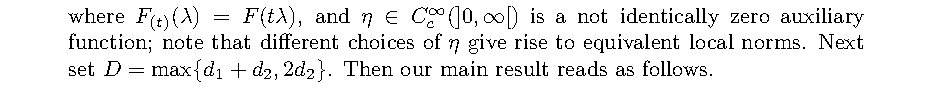
\includegraphics[width=0.81\linewidth]{figures/resolution_dimension.png}}
\par\medskip
\fbox{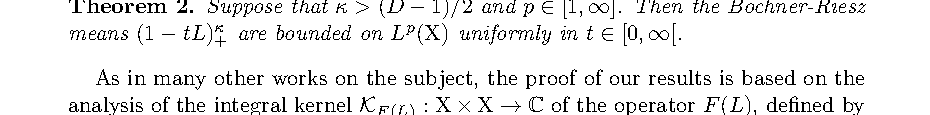
\includegraphics[width=0.81\linewidth]{figures/resolution_theorem.png}}
\caption{Two cropped excerpts: the definition of $D$ and Theorem 2 on page 2 of arXiv:1204.1159.}
\end{figure}

\clearpage
\section*{3. Parameter identification and implication}

The source operator is exactly the later operator with
\[
 d_1=n,\qquad d_2=1,\qquad x'=x,\qquad x''=t.
\]
Thus, for every $n\ge1$,
\[
 D=\max\{n+1,2\}=n+1.
\]
Substitution into \eqref{eq:MS} gives
\[
 \delta=\kappa>\frac{D-1}{2}=\frac n2.
\]
The scale parameters agree after putting $t=R^{-1}$:
$(1-tL)_+^\kappa=(1-G/R)_+^\delta=B_R^\delta$.
Consequently Martini--Sikora prove uniform boundedness on every
$L^p(\mathbb R^{n+1})$, including the source's range $1<p<\infty$, whenever
$\delta>n/2$. Since
\[
 \frac{n+1}{2}>\frac n2,
\]
this strictly implies the conjectured statement \eqref{eq:source}.

The supporting paper also states that its multiplier and Bochner--Riesz
thresholds are sharp when $d_1\ge d_2$.  Here $n=d_1\ge1=d_2$, so the later
result not only answers the source conjecture but identifies the stronger sharp
open-threshold range.

\section*{4. Provenance, search, and scope}

The four lightweight run indexes contained no entry for either arXiv id.
Bounded searches by the exact title, operator, and conjectured exponent found
arXiv:1204.1159. Its introduction explicitly compares its Theorems 1 and 2
with the earlier $d_2=1$ work, and its bibliography identifies that work as
Jotsaroop--Sanjay--Thangavelu.  The formula-level specialization above removes
any ambiguity caused by the supporting paper's nearby remark that Theorem 1
answers a different multiplier conjecture in the special case $d_1=d_2=1$.

No new proof is claimed here.  This packet records an exact primary-source
literature resolution and the parameter conversion showing that Theorem 2 is
strictly stronger than the queued conjecture.

\begin{thebibliography}{9}
\bibitem{JST}
K. Jotsaroop, P. K. Sanjay, and S. Thangavelu,
\emph{Riesz transforms and multipliers for the Grushin operator},
arXiv:1110.3227 (2011); J. Analyse Math. 119 (2013), 255--273.

\bibitem{MS}
A. Martini and A. Sikora,
\emph{Weighted Plancherel estimates and sharp spectral multipliers for the Grushin operators},
arXiv:1204.1159 (2012); Math. Res. Lett. 19 (2012), 1075--1088.
\end{thebibliography}

\end{document}
